\documentclass[12pt,a4paper]{article}
\usepackage[T1]{fontenc}
\usepackage[utf8]{inputenc}
\usepackage[brazil]{babel}
\usepackage{amsmath,amssymb,graphicx,booktabs,geometry,hyperref}
\geometry{margin=2.5cm}
\title{Modelagem e Busca Linear\\Paleta de cores e funções de teste}
\author{Tiago\\Ciência de Dados -- Universidade Federal do Ceará\\
Programação Não Linear -- Professor Ricardo Coelho}
\date{24 de outubro de 2026}

\begin{document}
\maketitle

\section{Parte 1: modelagem de uma paleta de três cores}

\subsection{Problema, dados e variáveis}
O problema é uma aplicação de \textbf{quantização de cores por agrupamento},
abordagem conhecida na literatura e discutida por Celebi~\cite{celebi2011}.
A modelagem apresentada é uma adaptação desse problema e de uma formulação
suave de agrupamento existente, não uma proposta matemática original.

Busca-se representar uma fotografia por três cores, minimizando o erro RGB
dos pixels. Utilizou-se a imagem \texttt{nascer do sol rio de janeiro.jpeg},
do acervo pessoal do autor. A original, de $3024\times4032$ pixels, foi
convertida para RGB e reduzida com LANCZOS para $192\times256$, preservando
a proporção. Cada componente foi dividida por 255, produzindo
$N=49\,152$ pixels fixos $p_i\in[0,1]^3$, com valores adimensionais.

As variáveis são as três cores $c_j=(R_j,G_j,B_j)^T$ da paleta:
\[
x=(R_1,G_1,B_1,R_2,G_2,B_2,R_3,G_3,B_3)^T\in\mathbb{R}^9.
\]

\subsection{Função objetivo irrestrita}
O erro por associação à cor mais próxima é
$E(x)=N^{-1}\sum_i\min_j\|p_i-c_j\|^2$.
Como esse mínimo pode não ser diferenciável nos empates, utiliza-se a forma
de energia livre do agrupamento por \textit{deterministic annealing}
apresentada por Rose~\cite[eq.~(25)]{rose1998}, especializada para este recorte:
\begin{equation}
\min_{x\in\mathbb{R}^9} f_\tau(x),\qquad
f_\tau(x)=-\frac{\tau}{N}\sum_{i=1}^N
\log\left[\frac13\sum_{j=1}^3
\exp\left(-\frac{\|p_i-c_j\|^2}{\tau}\right)\right],
\label{eq:objetivo}
\end{equation}
Na formulação de referência, tomam-se pesos dos dados iguais a $1/N$,
três representantes com pesos fixos $1/3$, distância quadrática no RGB
e temperatura $T=\tau$. Essas escolhas produzem a
Equação~\ref{eq:objetivo}. Aqui, $\tau=0{,}005$ permanece fixo e executa-se
um passo com Goldstein; não se implementa o processo completo de
redução gradual de temperatura de Rose. A aproximação é suave e satisfaz
$E\leq f_\tau\leq E+\tau\log3$, com
$\tau\log3\simeq0{,}00549306$. As exponenciais são avaliadas com
deslocamento pelo menor valor de distância, para estabilidade numérica.

O problema é irrestrito: projetar qualquer cor no cubo $[0,1]^3$ não aumenta
sua distância a nenhum pixel, portanto não aumenta o objetivo. Pela
continuidade e compacidade, existe um mínimo no cubo que também é global
no domínio irrestrito. Isso não garante que a busca local o alcance.
As variáveis não são recortadas durante a otimização.

\subsection{Gradiente e Hessiana}
Definindo $r_{ij}=c_j-p_i$ e
\[
q_{ij}=\frac{e^{-\|r_{ij}\|^2/\tau}}
{\sum_{\ell=1}^3e^{-\|r_{i\ell}\|^2/\tau}},
\]
a regra da cadeia fornece os blocos do gradiente:
\[
g_j=\nabla_{c_j}f_\tau=\frac2N\sum_iq_{ij}r_{ij}.
\]
Como
\[
\nabla_{c_k}q_{ij}=-\frac2\tau q_{ij}
(\delta_{jk}r_{ij}-q_{ik}r_{ik}),
\]
a regra do produto resulta nos blocos $3\times3$ da Hessiana:
\[
H_{jk}=\frac{2\delta_{jk}}N\sum_iq_{ij}I_3
-\frac4{N\tau}\sum_i(\delta_{jk}q_{ij}-q_{ij}q_{ik})r_{ij}r_{ik}^T.
\]
Empilham-se os três $g_j$ em um vetor e os nove $H_{jk}$ em uma matriz
$9\times9$. O delta $\delta_{jk}$ vale 1 para $j=k$ e 0 nos demais casos.
Diferenças centrais com $h=10^{-5}$, na paleta inicial e em uma paleta
perturbada, produziram erros absolutos máximos inferiores a
$4{,}15\times10^{-11}$ no gradiente e $1{,}43\times10^{-9}$ na Hessiana.

\subsection{Convexidade}
Sejam $\bar p$ a média dos pixels e
$S=N^{-1}\sum_i(p_i-\bar p)(p_i-\bar p)^T$.
No ponto $c_1=c_2=c_3=\bar p$, o gradiente é zero. Para
$v=(a,-a,0)$, com $\|a\|=1$,
\[
v^THv=\frac43-\frac8{3\tau}a^TSa.
\]
Escolhendo um autovetor de $\lambda_{\max}(S)=0{,}1368844167$,
obtém-se $v^THv=-71{,}6716889305<0$. Há também direções de curvatura
positiva nesse ponto; logo, ele é uma sela e $f_\tau$ não é globalmente
convexa. Na paleta inicial, a Hessiana é numericamente definida positiva
(menor autovalor $0{,}0092642542$), indicando convexidade estrita em uma
vizinhança suficientemente pequena, sem implicar convexidade global.

\subsection{Primeiro passo de descida}
A paleta inicial foi obtida ordenando os pixels pela média dos componentes
RGB e selecionando os percentis 10, 50 e 90. Cada linha das matrizes abaixo
é uma cor; $x_0$ e $x_1$ empilham suas linhas:
\[
C_0=\begin{pmatrix}
0{,}07843137&0{,}17647059&0{,}25490196\\
0{,}54901961&0{,}47843137&0{,}49019608\\
0{,}76470588&0{,}72941176&0{,}66666667
\end{pmatrix},
\]
\[
C_1=\begin{pmatrix}
0{,}12157864&0{,}20172708&0{,}26495457\\
0{,}54173215&0{,}48925441&0{,}49788293\\
0{,}74215063&0{,}71652582&0{,}66821411
\end{pmatrix}.
\]
Usou-se $d_0=-\nabla f_\tau(x_0)$, com
$g_0^Td_0=-\|g_0\|^2=-0{,}003507146131<0$.
A busca de Goldstein, implementada diretamente, usa $c_G=0{,}1$ e
aceitou a primeira tentativa $\alpha_0=1$. As duas condições foram satisfeitas:
\[
\underbrace{0{,}028970550720}_{f_0+(1-c_G)\alpha_0g_0^Td_0}
\leq f_\tau(x_1)=0{,}029618187484
\leq\underbrace{0{,}031776267624}_{f_0+c_G\alpha_0g_0^Td_0}.
\]
Assim, $x_1=x_0+\alpha_0d_0$ e
\[
f_\tau(x_0)=0{,}032126982237
>f_\tau(x_1)=0{,}029618187484,
\]
com redução de $7{,}8090\%$, sem recorte das variáveis.
O erro de reconstrução $E$, medido separadamente, passou de
$0{,}026729621032$ para $0{,}024228079500$.

\begin{figure}[htbp]
\centering
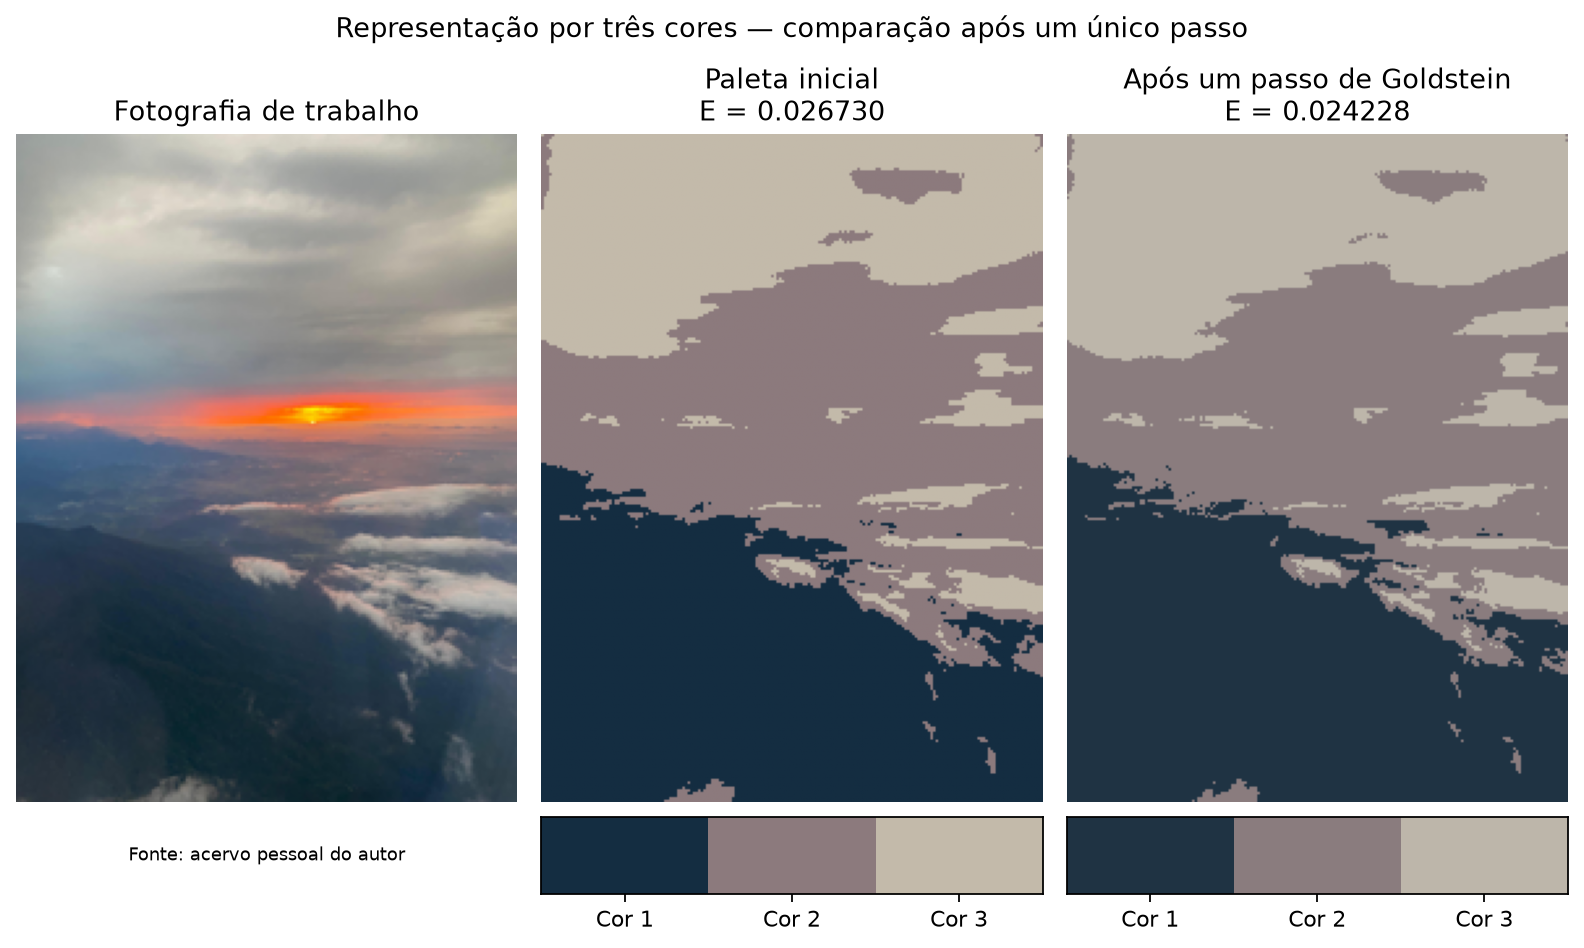
\includegraphics[width=\linewidth]{resultados/parte1/comparacao_primeiro_passo.png}
\caption{Fotografia de trabalho, reconstruções e paletas antes e após um
passo. Fonte da fotografia: acervo pessoal do autor.}
\end{figure}

A reconstrução mantém regiões gerais claras e escuras, mas perde detalhes
e os tons alaranjados. Uma única fotografia reduzida, uma paleta de três
cores e um passo limitam a fidelidade. O erro no RGB não é uma métrica
perceptual; redução do objetivo suave não garante melhora visual ou
otimalidade global. A convergência completa não é exigida nesta etapa.

\section{Parte 2: experimentos de busca linear}

\subsection{Funções de teste e parametrização unidimensional}
Foram executadas 27 combinações independentes: TP 1, TP 8 e TP 15,
três direções (G, N, M) e três buscas (Fibonacci, interpolação
quadrática/cúbica e Goldstein). Os pontos iniciais do enunciado são
$(8,9)$, $(0,0)$ e $(-1{,}2,1)$, respectivamente.

Para cada direção aplicada $d$, sejam $u(\alpha)=u_0+\alpha d_1$ e
$v(\alpha)=v_0+\alpha d_2$. As funções $\phi(\alpha)=f(x_0+\alpha d)$ são
\begin{align*}
\phi_1(\alpha)&=4[u(\alpha)-5]^2+[v(\alpha)-6]^2,\\
\phi_8(\alpha)&=\sum_{k=1}^3[b_k-u(\alpha)(1-v(\alpha)^k)]^2,
\quad b=(1{,}5,2{,}25,2{,}625),\\
\phi_{15}(\alpha)&=\{10[u(\alpha)-v(\alpha)^2]^2+[u(\alpha)-1]^2\}^{1/4}.
\end{align*}
As derivadas foram implementadas analiticamente e verificadas por diferenças
centrais nos pontos padrão e extras, com erros escalados inferiores a
$1{,}1\times10^{-10}$ no gradiente e $8{,}6\times10^{-11}$ na Hessiana.
A TP 15 não é diferenciável em $(1,1)$ e $(1,-1)$; o código rejeita suas
derivadas nesses pontos.

\subsection{Direções, métodos e parâmetros}
Com $g=\nabla f(x_0)$ e $H=\nabla^2f(x_0)$, calculam-se
\[
d_G=-g,\qquad Hd_N=-g,\qquad(H+\mu I)d_M=-g,
\]
resolvendo sistemas lineares, sem formar inversas. Adotou-se
\[
\delta=\max\{10^{-6},10^{-2}\max(1,\max_i|\lambda_i(H)|)\},\quad
\mu=\max(0,\delta-\lambda_{\min}(H)).
\]
A matriz modificada é definida positiva. A descida numérica exige
$g^Td<-10^{-12}\max(1,\|g\|\|d\|)$. Se Newton clássico falha, registra-se
o diagnóstico e aplica-se M, conforme o enunciado:
\begin{itemize}
\item TP 1: $\mu=0$; N e M coincidem.
\item TP 8: $d_N=(0,4{,}25)^T$, $g^Td_N=0$ e custo constante na linha;
usa-se M com $\mu\simeq1{,}3150671$.
\item TP 15: $d_N=(-4{,}4,0)^T$ e $g^Td_N\simeq2{,}7012172328>0$;
usa-se M com $\mu\simeq0{,}21697093$.
\end{itemize}
As seis linhas N substituídas por M pertencem à matriz de atribuição,
mas não representam sucesso da direção original nem trajetórias distintas
das linhas M correspondentes.

Para Fibonacci e interpolação, uma tentativa inicial 1 é reduzida pela
metade até diminuir o custo; depois é dobrada até obter $a<b<c$ com um
vale amostrado, limitado a 80 tentativas. Não se presume unimodalidade nem
mínimo global nas funções não convexas.

\begin{itemize}
\item \textbf{Fibonacci:} redução de intervalo com razões de números de
Fibonacci, reaproveitamento de avaliações e largura final $\leq10^{-7}$.
A última comparação evita gerar pontos coincidentes.
\item \textbf{Interpolação Q/C:} alterna mínimos de quadráticos interpoladores
e cúbicos de Hermite; candidatos inadequados são substituídos por um ponto
médio. Parada: largura $\leq10^{-7}\max(1,|\alpha|)$ ou 300 tentativas.
\item \textbf{Goldstein:} verifica ambas as desigualdades com $c_G=0{,}1$,
tentativa inicial 1, expansão/redução e limite de 100 tentativas.
\end{itemize}
As buscas foram implementadas sem rotinas prontas e conferidas em
quadráticas com mínimos conhecidos. Na TP 1, a referência analítica é
$\alpha_*=-g^Td/(d^THd)$. Cada caso parte de seu próprio $x_0$ e retorna
um único próximo ponto $x_1=x_0+\alpha d$.

\subsection{Resultados e discussão}
As tabelas apresentam os 27 casos. N/M indica N solicitado e M aplicado;
f/g conta avaliações de custo/gradiente direcional, incluindo o intervalo
e o custo em zero, com reaproveitamento por cache. As derivadas iniciais
usadas para formar as direções não entram nesses contadores. A rotina de
gradiente do cúbico também retorna a Hessiana, embora a busca não a use.
\begin{table}[htbp]
\centering
\small
\caption{TP 1: nove casos padrão; custo inicial $45$.}
\begin{tabular}{llrlrr}
\toprule
Sol./usada & Busca & $\alpha$ & $x_1=(u_1,v_1)$ & $f(x_1)$ & f/g \\
\midrule
G/G & Fib. & $0{,}13076922$ & $(4{,}86154; 8{,}21538)$ & $4{,}9846154$ & 39/0 \\
G/G & Q/C & $0{,}13076923$ & $(4{,}86154; 8{,}21538)$ & $4{,}9846154$ & 38/29 \\
G/G & Gold. & $0{,}125$ & $(5; 8{,}25)$ & $5{,}0625$ & 5/0 \\
N/N & Fib. & $1$ & $(5; 6)$ & $3{,}9443045\times10^{-30}$ & 40/0 \\
N/N & Q/C & $1$ & $(5; 6)$ & $0$ & 52/48 \\
N/N & Gold. & $1$ & $(5; 6)$ & $0$ & 2/0 \\
M/M & Fib. & $1$ & $(5; 6)$ & $3{,}9443045\times10^{-30}$ & 40/0 \\
M/M & Q/C & $1$ & $(5; 6)$ & $0$ & 52/48 \\
M/M & Gold. & $1$ & $(5; 6)$ & $0$ & 2/0 \\
\bottomrule
\end{tabular}
\end{table}

\begin{table}[htbp]
\centering
\small
\caption{TP 8: nove casos padrão; custo inicial $14{,}203125$.}
\begin{tabular}{llrlrr}
\toprule
Sol./usada & Busca & $\alpha$ & $x_1=(u_1,v_1)$ & $f(x_1)$ & f/g \\
\midrule
G/G & Fib. & $0{,}16666667$ & $(2{,}125; 0)$ & $0{,}65625$ & 38/0 \\
G/G & Q/C & $0{,}16666667$ & $(2{,}125; 0)$ & $0{,}65625$ & 48/43 \\
G/G & Gold. & $0{,}25$ & $(3{,}1875; 0)$ & $4{,}0429688$ & 4/0 \\
N/M & Fib. & $0{,}020386452$ & $(0{,}5515; -1{,}25811)$ & $7{,}6282475$ & 36/0 \\
N/M & Q/C & $0{,}020386444$ & $(0{,}5515; -1{,}25811)$ & $7{,}6282475$ & 28/13 \\
N/M & Gold. & $0{,}0234375$ & $(0{,}634038; -1{,}4464)$ & $8{,}6656561$ & 9/0 \\
M/M & Fib. & $0{,}020386452$ & $(0{,}5515; -1{,}25811)$ & $7{,}6282475$ & 36/0 \\
M/M & Q/C & $0{,}020386444$ & $(0{,}5515; -1{,}25811)$ & $7{,}6282475$ & 28/13 \\
M/M & Gold. & $0{,}0234375$ & $(0{,}634038; -1{,}4464)$ & $8{,}6656561$ & 9/0 \\
\bottomrule
\end{tabular}
\end{table}

\begin{table}[htbp]
\centering
\small
\caption{TP 15: nove casos padrão; custo inicial $2{,}701217233$.}
\begin{tabular}{llrlrr}
\toprule
Sol./usada & Busca & $\alpha$ & $x_1=(u_1,v_1)$ & $f(x_1)$ & f/g \\
\midrule
G/G & Fib. & $1{,}2043933$ & $(-0{,}460607; -0{,}34435)$ & $1{,}5305656$ & 41/0 \\
G/G & Q/C & $1{,}2043933$ & $(-0{,}460607; -0{,}34435)$ & $1{,}5305656$ & 30/18 \\
G/G & Gold. & $1$ & $(-0{,}586087; -0{,}116205)$ & $1{,}5722581$ & 2/0 \\
N/M & Fib. & $0{,}018489479$ & $(0{,}368385; 0{,}565943)$ & $0{,}80601955$ & 36/0 \\
N/M & Q/C & $0{,}018489492$ & $(0{,}368386; 0{,}565942)$ & $0{,}80601955$ & 24/12 \\
N/M & Gold. & $0{,}03125$ & $(1{,}45081; 0{,}266378)$ & $2{,}0944431$ & 7/0 \\
M/M & Fib. & $0{,}018489479$ & $(0{,}368385; 0{,}565943)$ & $0{,}80601955$ & 36/0 \\
M/M & Q/C & $0{,}018489492$ & $(0{,}368386; 0{,}565942)$ & $0{,}80601955$ & 24/12 \\
M/M & Gold. & $0{,}03125$ & $(1{,}45081; 0{,}266378)$ & $2{,}0944431$ & 7/0 \\
\bottomrule
\end{tabular}
\end{table}

Todos os casos produziram redução estrita. Na TP 1, N e M atingiram
$(5,6)$ com passo igual ou numericamente próximo de 1; o resíduo de
Fibonacci é de arredondamento. Na TP 8, G mantém $v=0$ e o mínimo da linha
ocorre em $\alpha=1/6$, com custo $0{,}65625$, inferior ao dos passos
regularizados neste experimento. Na TP 15, a regularização evita uma
direção de subida; Fibonacci e Q/C produziram custos próximos entre si.

Goldstein satisfez ambas as desigualdades nos nove casos, mas pode retornar
redução menor por aceitar um passo suficiente em vez de minimizar a linha.
Nos nove casos de cada busca, Fibonacci usou 342 avaliações de custo;
Q/C, 324 de custo e 236 de gradiente; Goldstein, 47 de custo.
Como os critérios de precisão e os custos de cada avaliação diferem,
esses totais não demonstram superioridade universal de um método.

\subsection{Testes extras}
Foram executados mais 27 casos, sem substituir os obrigatórios, nos pontos
TP 1: $(4,2)$; TP 8: $(1,0{,}5)$; TP 15: $(-0{,}5,0{,}5)$.
Todos apresentaram redução e valores finitos:
\begin{center}
\begin{tabular}{lrr}
\toprule
Função & Menor redução (\%) & Maior redução (\%)\\
\midrule
TP 1 & 60,0000 & 100,0000\\
TP 8 & 62,8727 & 94,7387\\
TP 15 & 28,1026 & 53,4136\\
\bottomrule
\end{tabular}
\end{center}
Os próximos pontos e diagnósticos extras estão no CSV/JSON. Os testes
avaliam o primeiro passo; não provam convergência para qualquer inicialização.

\section{Manual de uso}
\begin{enumerate}
\item Instale Python 3 e as dependências e abra o Jupyter:
\begin{verbatim}
python -m pip install numpy pillow matplotlib notebook
python -m notebook
\end{verbatim}
\item Mantenha os dois notebooks e a fotografia na pasta do trabalho.
Abra \texttt{parte 1.ipynb} ou \texttt{parte 2.ipynb} e execute todas as
células em ordem após reiniciar o kernel. Os notebooks são independentes.
\item \textbf{Entradas da Parte 1:} \texttt{NOME\_IMAGEM} indica o arquivo;
\texttt{LADO\_MAXIMO}=256 controla a resolução; \texttt{TAU}=0,005
controla a suavização. A paleta é inicializada deterministicamente.
\item \textbf{Entradas da Parte 2:} \texttt{PROBLEMAS} contém funções e
pontos iniciais; \texttt{PARAMETROS} contém tolerâncias, regularização e
limites. Os padrões são os descritos na seção de experimentos.
\item \textbf{Saídas:} as células mostram imagens, tabelas e diagnósticos.
\texttt{resultados/parte1} contém as reconstruções e
\texttt{resultado\_primeiro\_passo.json}.
\texttt{resultados/parte2} contém
\texttt{resultados\_obrigatorios.csv}, \texttt{resultados\_extras.csv},
\texttt{experimentos.json}, resumo e gráficos.
\item Nas tabelas, leia direção solicitada/usada, passo, próximo ponto,
custos, redução e avaliações. O JSON inclui parâmetros e históricos
completos; use-o ou o CSV para valores com maior precisão que os arredondados
neste relatório. Falhas têm diagnóstico explícito. Gradiente numericamente
nulo gera status \texttt{estacionario}, passo zero e nenhuma busca, sem
exigir redução estrita ou afirmar mínimo global.
\end{enumerate}
\paragraph{Teste interativo opcional.}
O notebook \texttt{testar\_paleta.ipynb} permite escolher outra imagem
sem executar os notebooks das Partes 1 e 2:
\begin{enumerate}
\item Abra o arquivo no Jupyter ou no VS Code com suporte a notebooks
e selecione um kernel Python 3. Pelo terminal, na pasta do trabalho,
também é possível abrir com:
\begin{verbatim}
python -m notebook testar_paleta.ipynb
\end{verbatim}
\item Execute todas as células em ordem. A primeira verifica e instala
apenas as dependências ausentes: NumPy, Pillow, Matplotlib e ipywidgets.
A instalação requer internet. Mantenha o kernel ativo para usar o painel.
\item Clique em ``Escolher imagem'', selecione o arquivo no computador
e clique em ``Gerar paleta''. Para testar a imagem original, use
``Usar foto do trabalho'', quando ela estiver disponível na pasta.
\item Observe a imagem de trabalho, a reconstrução e as três cores em
RGB (0 a 255) e hexadecimal. Para copiar os valores, selecione o texto
na caixa de cores e pressione Ctrl+C. Para outra imagem, repita o upload.
\item Como alternativa ao painel, remova o comentário da chamada
\texttt{testar\_arquivo("minha\_foto.jpeg")} na última célula e informe
um caminho acessível ao computador do kernel.
\end{enumerate}
A ferramenta executa o mesmo primeiro passo da Parte 1, sem alterar os
resultados do trabalho; não busca convergência completa. O resultado fica
na variável \texttt{ultimo\_resultado}. Imagens com poucas cores podem
retornar cores repetidas; gradiente nulo retorna a paleta sem busca.

As saídas são atualizadas a cada execução, sem sobrescrever a fotografia.
PNG usa RGB de 8 bits; os cálculos e JSON mantêm ponto flutuante.
O ambiente verificado utilizou Python 3.11.9, NumPy 2.4.6, Pillow 12.3.0
e Matplotlib 3.11.2.

\appendix
\section{Auditoria de uso de IA}
\subsection{Resumo das solicitações}
A IA foi utilizada para interpretar o enunciado, planejar o projeto,
explorar temas, preparar a fotografia, formular o objetivo e suas
derivadas, implementar as duas partes, verificar resultados e revisar o
código. Também auxiliou na redação e implementou a ferramenta independente
de teste de imagens, solicitada posteriormente. A escolha do tema e a fotografia são
do autor. Os resumos das solicitações efetivamente registradas são:
\begin{enumerate}
\item compreender o trabalho e organizar o planejamento;
\item explorar aplicações de otimização e escolher a paleta de cores;
\item preparar a imagem e finalizar a implementação da Parte 1;
\item implementar e verificar os experimentos da Parte 2;
\item revisar as duas partes e registrar os erros e suas correções.
\end{enumerate}
O histórico está em \texttt{resumo de prompts.md}; os exemplos de
prompts para estudo ali identificados não são tratados como interações
realizadas. As contribuições estão descritas neste apêndice, e os erros
detalhados constam de \texttt{auditoria critica de erros.md}.

\subsection{Erro de implementação: omissão de pontos estacionários}
O código gerado pela IA retornava uma lista vazia de direções quando a
norma do gradiente era $\leq10^{-12}$. O executor apenas percorria essa
lista e omitia as nove combinações da função. O erro foi identificado
testando a TP 1 em $(5,6)$: o total caiu de 27 para 18 registros.

A análise mostrou que $\nabla f_1(5,6)=0$ e $f_1(5,6)=0$; as direções são
nulas e $\phi(\alpha)=0$. Logo, redução estrita é impossível, e não se deve
forçar uma busca de descida nem omitir o caso.
A correção em \texttt{executar\_casos} preserva os nove registros com
status \texttt{estacionario}, passo zero, ponto e custo inalterados e
nenhuma busca. Goldstein fica não aplicável; não se afirma que todo ponto
estacionário seja um mínimo.

O teste de regressão confirmou 27 registros, nove estacionários da TP 1,
sem iterações de busca. O ponto inicial original foi restaurado, e ambos
os notebooks foram reexecutados sem erros. Os resultados originais da
Parte 1 e dos 54 casos da Parte 2 permaneceram idênticos.

Também ocorreram dois erros de sintaxe ao gerar textos das células, com
strings não encerradas. Foram corrigidos removendo substituições
redundantes de barras invertidas e usando \texttt{chr(10).join(texto)}
na exportação do resumo. Os diagnósticos e as validações estão no arquivo
de auditoria. A ausência de descida de Newton nas TP 8 e TP 15 é uma
propriedade matemática tratada pelo algoritmo, não um erro da IA.

\begin{thebibliography}{9}
\bibitem{celebi2011} CELEBI, M. Emre. Improving the Performance of K-Means
for Color Quantization. \textit{Image and Vision Computing}, v.~29,
p.~260--271, 2011. DOI: \href{https://doi.org/10.1016/j.imavis.2010.10.002}
{10.1016/j.imavis.2010.10.002}.
Versão disponível em: \url{https://arxiv.org/abs/1101.0395}.
\bibitem{rose1998} ROSE, Kenneth. Deterministic Annealing for Clustering,
Compression, Classification, Regression, and Related Optimization Problems.
\textit{Proceedings of the IEEE}, v.~86, n.~11, p.~2210--2239, 1998.
Disponível em: \url{https://scl.ece.ucsb.edu/sites/default/files/publications/b98_2_0.pdf}.
\bibitem{enunciado} COELHO, Ricardo. \textit{Primeiro Projeto Computacional:
Modelagem e Busca Linear}. Programação Não Linear, UFC, 2026. Enunciado
disponibilizado pelo professor.
\bibitem{foto} TIAGO. \textit{Nascer do sol no Rio de Janeiro}. Fotografia
digital, acervo pessoal do autor; data de captura não informada.
\end{thebibliography}
\end{document}
